\documentclass[
	12pt,
	a4paper,
	abstract,
	bibliography=totoc,
	chapterprefix,
	headings=openright,
	numbers=endperiod,
	parskip=half,
	twoside,
]{scrreprt}

\usepackage[T1]{fontenc}
\usepackage[utf8]{inputenc}

\usepackage{libertinus}
\usepackage[varqu,scaled=0.95]{inconsolata}
\usepackage{newtxmath}

\usepackage[english]{babel}

% Use less space for the page number
\usepackage[margin=2.5cm,footskip=36pt]{geometry}
\usepackage{graphicx}
\usepackage[htt]{hyphenat}
\usepackage{listings}
% insert for rust syntax highlighting for listings
\usepackage{listings-rust}
\lstset{language=Rust}
% ---------
\usepackage{microtype}
\usepackage{subcaption}
% Required for listings's upquote
\usepackage{textcomp}
\usepackage{upquote}
\usepackage{xcolor}

\usepackage[hyphens]{url}
\usepackage[hidelinks,pagebackref]{hyperref}
\usepackage[capitalise,noabbrev]{cleveref}

\usepackage[color=ovgu-orange]{todonotes}

\usepackage{lipsum}

\graphicspath{{./figures/}}

\definecolor{ovgu-blue}{HTML}{0068B4}
\definecolor{ovgu-darkgray}{HTML}{606060}
\definecolor{ovgu-lightgray}{HTML}{C0C0C0}
\definecolor{ovgu-orange}{HTML}{F39100}
\definecolor{ovgu-purple}{HTML}{7A003F}
\definecolor{ovgu-red}{HTML}{D13F58}

\lstset{
	basicstyle=\ttfamily,
	commentstyle=\color{ovgu-darkgray},
	keywordstyle=\color{ovgu-blue},
	numberstyle=\ttfamily\color{ovgu-darkgray},
	stringstyle=\color{ovgu-purple},
	rulecolor=\color{ovgu-lightgray},
	frame=single,
	numbers=left,
	language=C,
	breaklines=true,
	breakatwhitespace=true,
	postbreak=\hbox{$\hookrightarrow$ },
	showlines=true,
	showstringspaces=false,
	upquote=true,
	tabsize=4,
	gobble=0,
	captionpos=b,
	abovecaptionskip=\medskipamount,
}

\renewcommand*{\backref}[1]{}
\renewcommand*{\backrefalt}[4]{%
\ifcase #1%
{\color{ovgu-darkgray}(\color{ovgu-red}Not~cited\color{ovgu-darkgray})}%
\or%
{\color{ovgu-darkgray}(Cited~on~page~#2)}%
\else%
{\color{ovgu-darkgray}(Cited~on~pages~#2)}%
\fi%
}

\titlehead{\centering
\includegraphics[width=0.66\textwidth]{OVGU-INF}}

\subject{Bachelor/Master Thesis}
\title{Title}

\author{
Author\\
{\large\href{mailto:christian.grueneberg@st.ovgu.de}{\nolinkurl{christian.grueneberg@st.ovgu.de}}}
}

\date{\today}

\publishers{
First Reviewer:\\
Prof. Dr. Michael Kuhn

\medskip

Second Reviewer:\\
Johannes Wünsche

\medskip

Supervisor:\\
Johannes Wünsche
}

\begin{document}

% \frontmatter
\pagenumbering{roman}

\maketitle

\begin{abstract}

% abstract als letztes schreiben, fast kurz die Arbeit zusammen um schnell einen Überblick zu geben
% enthält den wesentlichen Inhalt und die kurz zusammengefasst das Ergebnis der Arbeit
% stellt heraus was der eigene Anteil war/ist
% ca 1 Seite

-> write this last after everything else

\end{abstract}

\tableofcontents

% \mainmatter
\cleardoubleoddpage
\pagenumbering{arabic}

\chapter{Introduction}
\label{cha:introduction}

% Was ist das Problem und warum ist es wichtig.
% stellt heraus warum der Leser sich dafür interessieren sollte
% die Motivation hinter der Arbeit
% beinhaltet auch was ist neu, was habe ich neues zum Thema beigetragen
% was sind die Ergebnisse,
% es wird auch kurz dargestellt wie vorgeganngen wurde
% der Aufbau der Arbeit wird kurz vorgestellt

% 5%-19% 2-4

% possible structure
\section{Memory Hierarchy}
Since the invention of integrated circuits in 1959, CPU performance has grown faster than main memory performance.
Figure \ref{fig:processor memory gap} shows the improvement in processor performance and DRAM performance since the 1980s.
This leads to the "processor-memory performance gap", also known as the "memory wall" problem \cite{wulf1995hitting}.
One of the reasons for this is that in the semiconductor industry, CPU and memory are separate domains and have been optimized for different goals.
CPUs have been optimized for higher clock frequency, whereas DRAM and hard disks have been optimized primarily for higher memory capacity \cite{cpu-mem-gap}.
Even though the rates of increase in single-core performance have slowed down and thus the performance gap between processor and memory is growing more slowly, the use of multi-core processors has increased the bandwidth requirements so that the main memory must support more memory accesses.

\begin{figure}[ht]
	\centering
	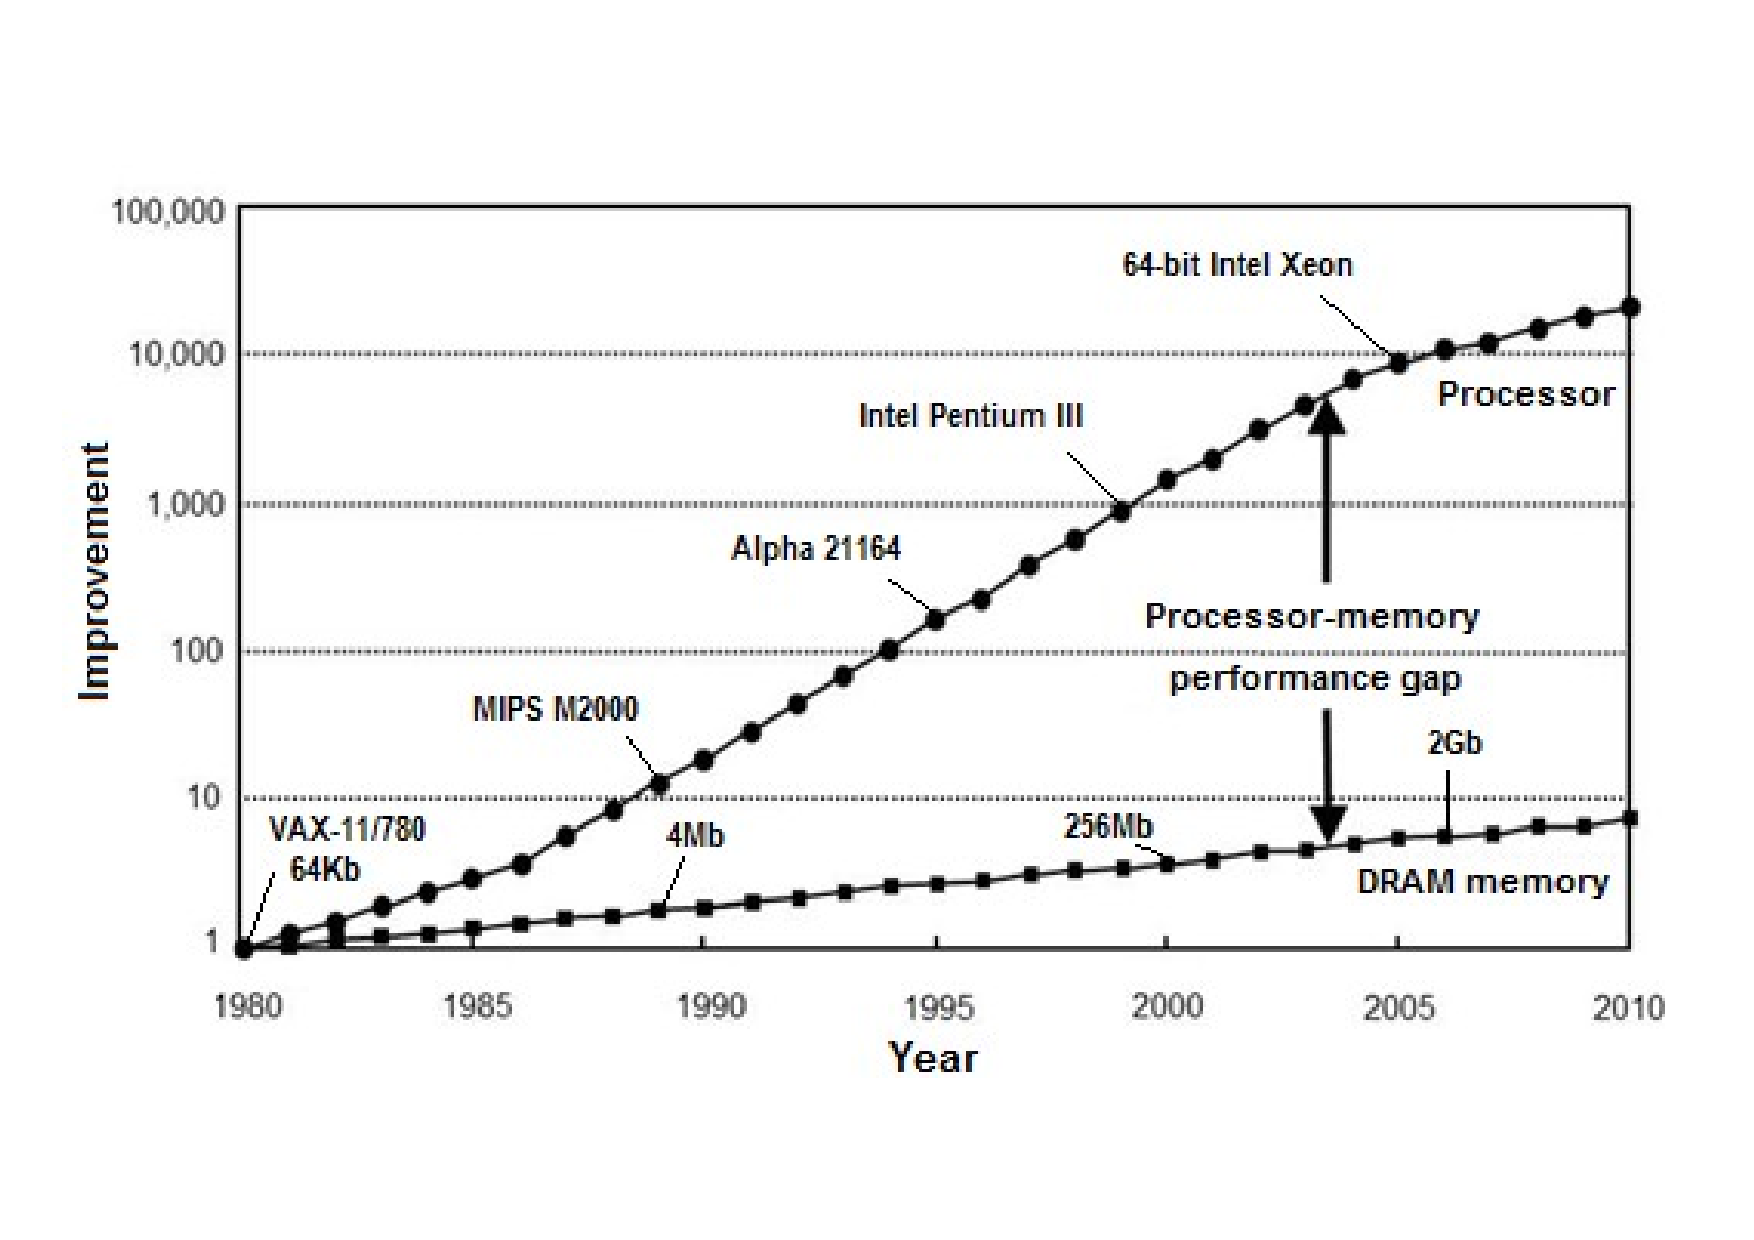
\includegraphics[scale=0.45]{processor_memory_gap.pdf}
	\caption{Processor-Memory gap, figure from \cite{cpu-mem-gap}}
		\label{fig:processor memory gap}
\end{figure}


To reduce the processor-memory performance gap, memory is built up hierarchically, as shown in figure \ref{fig:memory hierarchy}.
The memory is ordered from fast, expensive and low capacity, which is close to the processor, to progressively slower, cheaper and higher capacity, which is further away from the processor.
The goal of the memory hierarchy is to develop systems that have enough fast memory, CPU cache and DRAM to not slow down the CPU significantly and on the other hand, have as much memory capacity as necessary provided by using hard disks, solid state disk or flash memory without excessive costs.

\begin{figure}[ht]
	\centering
	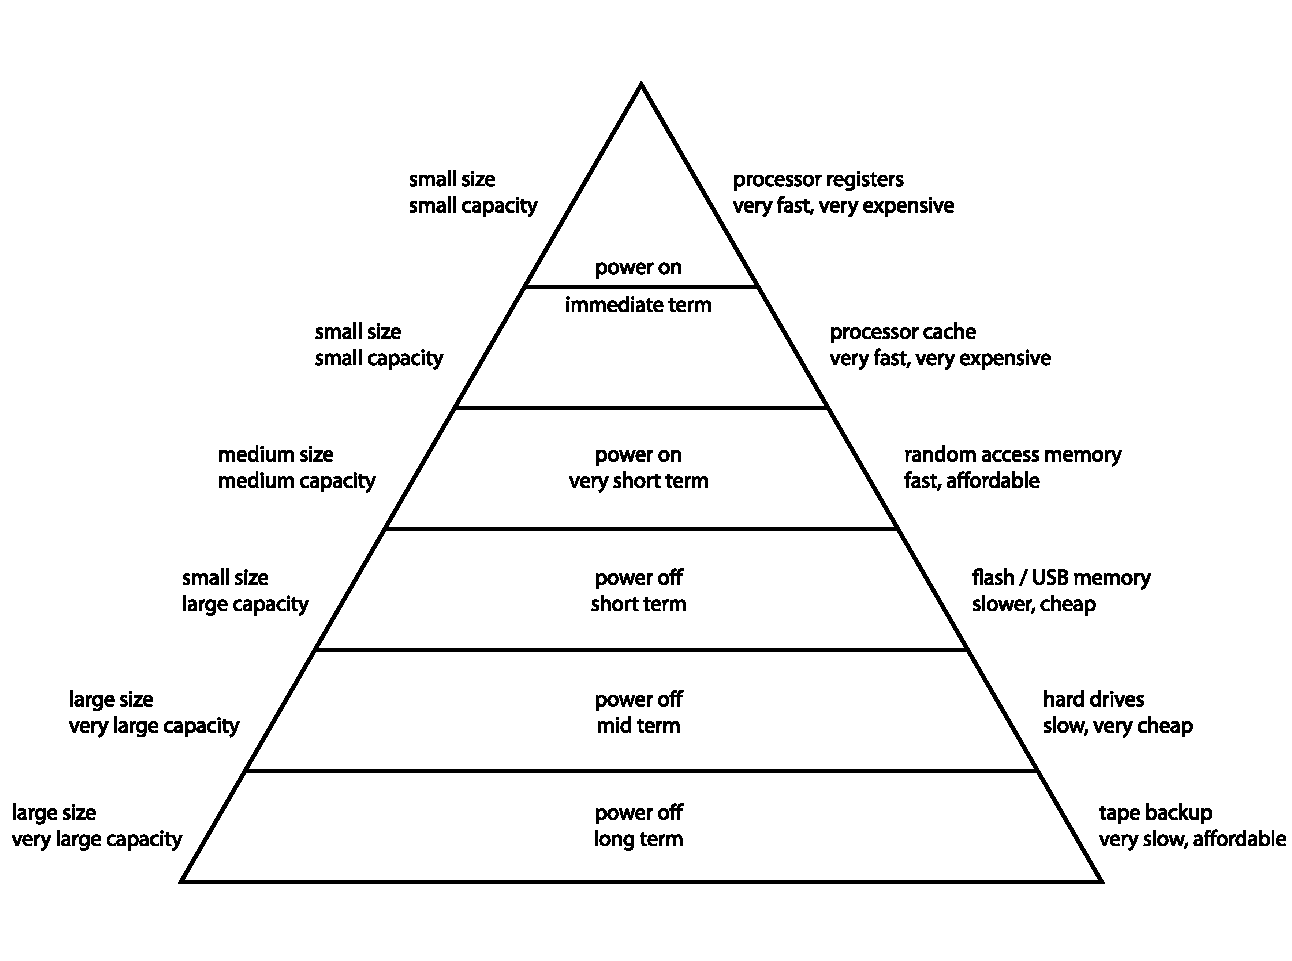
\includegraphics[scale=0.6]{ComputerMemoryHierarchy.pdf}
	\caption{Memory Hierarchy}
		\label{fig:memory hierarchy}
\end{figure}
\todo[inline]{check how to cite online sources, it is from wikipedia https://upload.wikimedia.org/wikipedia/commons/9/9d/ComputerMemoryHierarchy.png}



\section{Contribution}
% check if contribution or contributions is right
- new is direct comparison of clock based cache replacement algorithms\\

\section{Outline}
- description of the structure of the following work\\

% 5-10%, ca. 2-5 Seiten 

\chapter{Background}
\label{cha:background}

% darstellen der nötigen Informationen und Arbeiten um die weitere Arbeit verstehen zu können
% nicht zu weit ausschweifen
% 10-20%, ca. 4-10 Seiten

- next chapter gives a short overview of topics necessary to understand the following work\\

\section{$B^{\epsilon}$-tree}

% own section for $B^{\epsilon}$-tree
%The $B^{\epsilon}$-tree is a write-optimized version of the B-tree, which are widely used for filesystems or databases, with better performance for insert, range queries and key-value updates \cite{bender2015introduction}.
%Unlike the B-tree, the $B^{\epsilon}$-tree has a buffer for each node, where changes to the subtree associated with the node are stored and
%only when the buffer overflows, the changes are written to the nodes of the subtree, which reduces the number of write operations and the data fragmantation.

The idea for the $B^{\epsilon}$-tree was introduced by \cite{brodal2003lower} in a study of the trade off between insertions and queries for comparison-based external memory dictionaries.

The basis for $B^{\epsilon}$-trees is the B-tree, which has good performance on queries but suffers from poor performance on small writes, as shown in \cite{bender2015introduction}, 
because the entire node must be updated for each small write.
However, if we reduce the node size to optimize for small writes, sequential read performance suffers because many smaller nodes have to be fetched from disk instead of fewer but larger ones.

To optimize for both cases, the $B^{\epsilon}$-tree adds a buffer to each internal node of size $B - B^{\epsilon} $ with $ 0 \leq \epsilon < 1$ as shown in figure \ref{fig:structure B-epsilon-tree}.

\begin{figure}[ht]
	\centering
	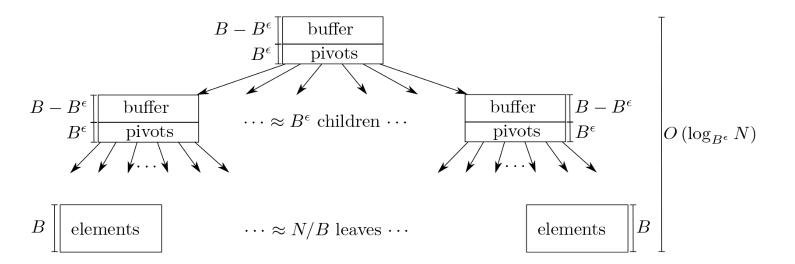
\includegraphics[scale=0.6]{B-epsilon_structure.png}
	\caption{Structure $B^{\epsilon}$-tree from \cite{bender2015introduction}}
		\label{fig:structure B-epsilon-tree}
\end{figure}

As new data is inserted into the $B^{\epsilon}$-tree, the data is written to the buffer of the root node as "insert message".
Only when the root node's buffer is full, a batch of messages is flushed down the tree, preferably to the node with the most pending messages. 
If a node needs to be split, the buffer is also split between the new nodes.
When the insert message arrives at a leaf node, the data is added to the leaf.

This behavior leads to better insertion performance than B-trees, since insertion always occurs at the root, no searching for the correct insertion point is required, and  
the actual writing of data is delayed in batches only when enough changes have accumulated in a buffer.
On deletion a "tombstone message" will be insert into the tree and will be flushed down the tree to a leaf, like an insertion message.

For queries, in the $B^{\epsilon}$-tree, we also need to check buffer on the way to the leaf nodes to see if there are any relevant messages.
These messages must be processed, but that does not mean they are flushed down immediately, this can happen later.

So the $B^{\epsilon}$-trees achieves similar asymptotic I/O cost for queries but is better for insertions compared to B-trees.
\todo[inline]{write a bit more detailed about this}


\section{Haura}
%- introduce haura storage stack and explain structure\\
%- short explaination B-epsilon-tree\\
%- task of the cache\\

\todo[inline]{check definition for haura with Johannes}

Haura is a research storage stack written primarily in Rust.
Unlike traditional file systems, haura runs in user space rather than kernel space.
Also, haura uses a key-value and object interface rather than the usual POSIX interface.
It can be used either directly by an application, in which case haura runs in the process context of the application, or
use JULEA as a wrapper for haura.
JULEA then runs the haura instance detached from the user applications, which means that the user application can be terminated or new applications can be created as long as JULEA is running, resulting in more flexibility compared to direct use.

\todo[inline]{insert schemes from haura docu for better understanding}
\todo[inline]{insert link to haura docu as source}
\todo[inline]{epsilon is written diffrently then in original paper}

The development of Haura started to compare $B^{\epsilon}$-tree to ZFS and ext4 filesystem \cite{wiedemann2018modern}, where the haura stack
achieved an improved write performance especially for small random write workloads and better sequential throughput.
Then Haura would be extended by \cite{hoppner2021design} to support multiple storage levels
The work of \cite{hoppner2021design} extended Haura with an object storage interface and the support of multiple storage levels while preserving the benefits of the $B^{\epsilon}$-tree.

As pointed out by \cite{wunsche2022data} the advantage of Haura is that all levels which a relevant to implement and optimize a storage stack a combined in a single code base, so that it is easy change subsystems and test different approaches.
Haura is structured in layers as shown in figure \ref{fig:structure haura}.

\begin{figure}[ht]
	\centering
	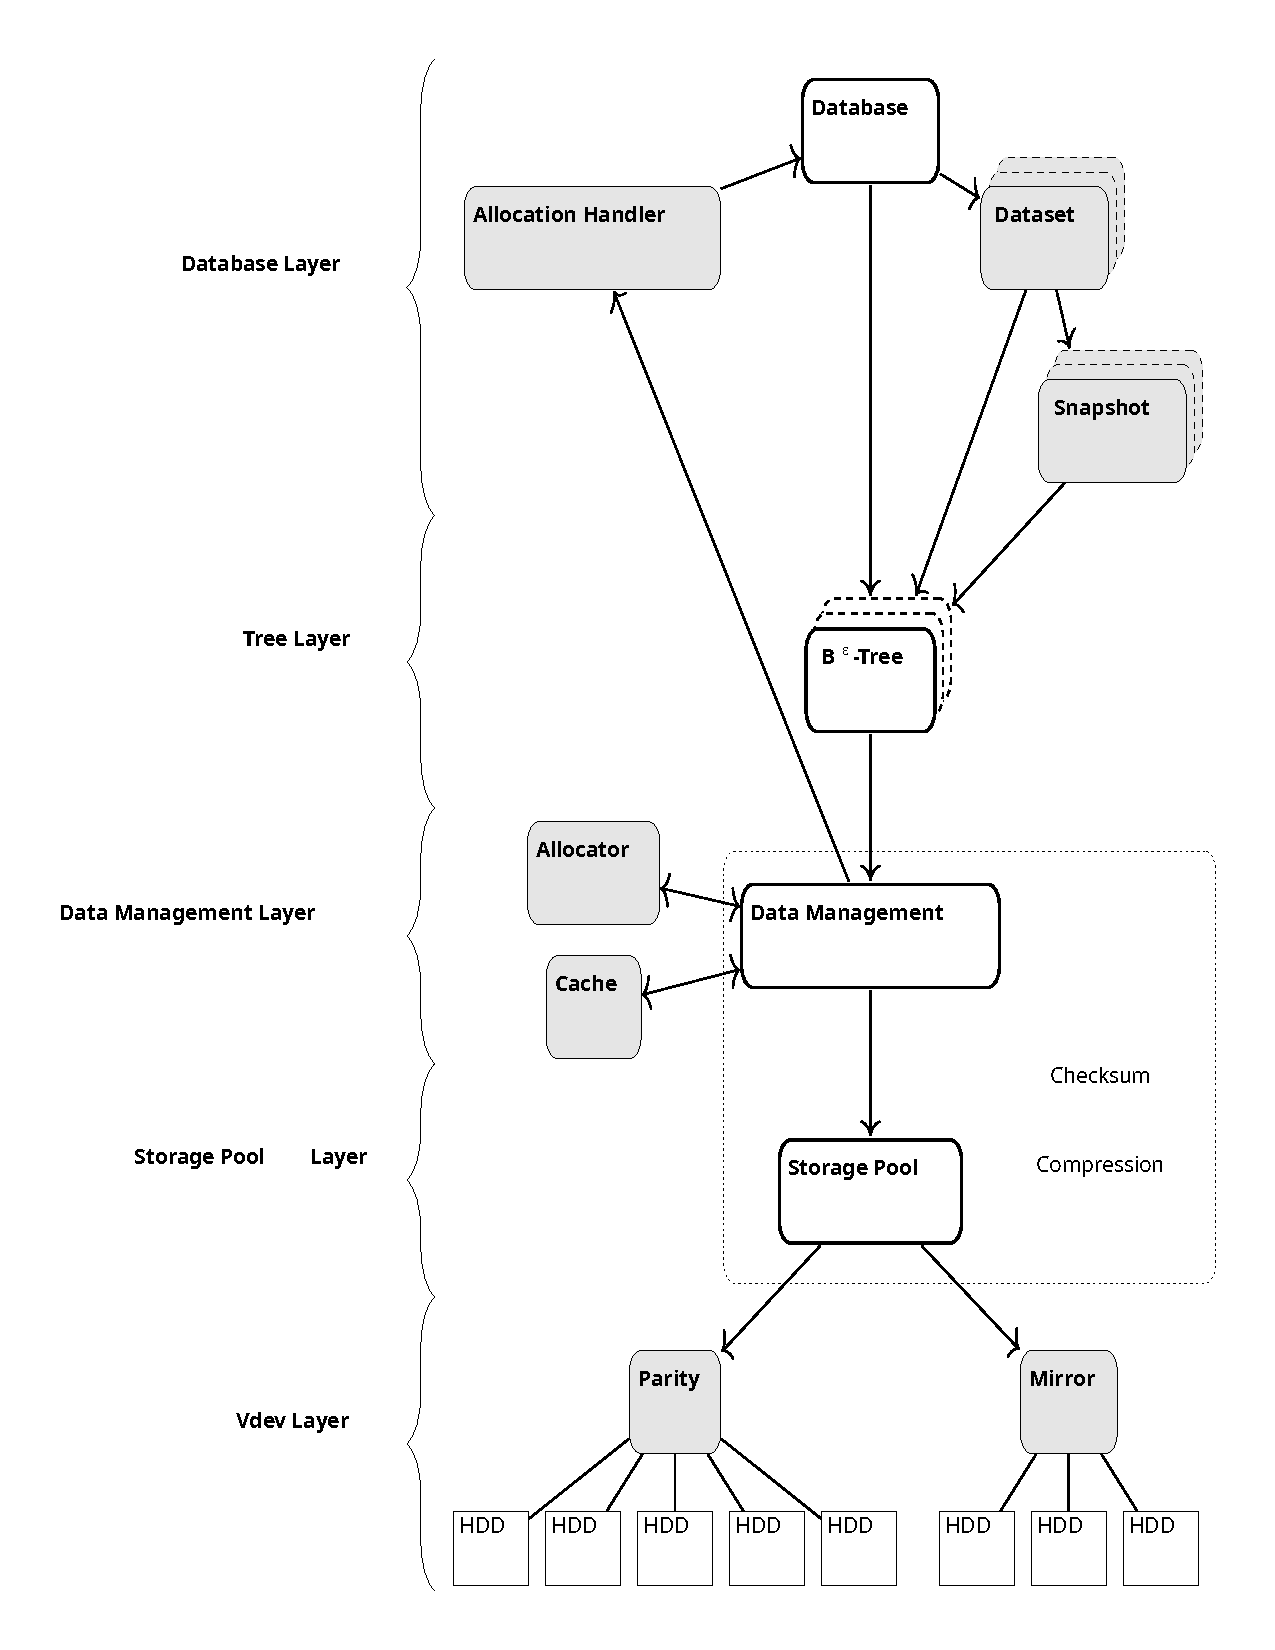
\includegraphics[scale=0.4]{overview_haura_level.pdf}
	\caption{Structure haura, from \cite{wiedemann2018modern}}
		\label{fig:structure haura}
\end{figure}
\todo[inline]{check were I have to put the source for the figure, in text or under the figure}


At the top is the \emph{Database Layer} which manages multiple datasets and snapshots. Each dataset provide a key-value interface, snapshots only read-only key-value interface. Also for each dataset exists an own $B^{\epsilon}$-tree and  a root tree which saves the allocation bitmaps and metadata.

The next layer, the \emph{Tree Layer} manages the $B^{\epsilon}$-trees.
The \emph{database layer} sends messages to the $B^{\epsilon}$ trees consisting of key-value or key-message pairs that the $B^{\epsilon}$ trees process. A message for key-message pair can contain arbitrary data or apply arbitrary code on data.
Key-value pairs are stored in leave nodes and key-message nodes are stored in inner nodes of the tree.
Each node is an object for the \emph{Data Management Layer} and is tracked individually.

The \emph{Data Management Layer}(DML) manages objects for the \emph{Tree Layer} and \emph{database layer} which means cache objects in memory, 
track modifications to objects and write-back modified objects.
Main part of the DML is the Data Management Unit (DMU).
The DMU is shared by all trees and ensures that no irregular state can be reached.
It takes care of critical disk management such as block allocation.
In addition, the DMU manages the cache, which is the main topic of this work.

The \emph{Storage Pool Layer} is an abstraction over the used storage hardware.
Furthermore the storage is divided in to tiers from \emph{Fastest}, \emph{Fast}, \emph{Slow} to \emph{Slowest}.
The user can decide how the used hardware falls into these tiers. Also, not all tiers need to be used.

The last layer, the \emph{Vdev Layer}, is responsible for actually reading and writing data from the disks.
Single disk, multiple disks or RAID-like configurations can be used.

\section{Caching}
%Due to the use of a memory hierarchy, caching is used in several places, as shown in table \ref{tab:caching hierarchy} and can either be handle in hardware like the L1 and L2 cache of a cpu-core, in software like a web cache or a combination of both.

Closely related to the memory hierarchy is caching.
Caching refers to a fast and smaller primary memory in front of a larger but slower secondary memory, so that requested data can be served faster from the primary memory instead of fetching the data from the slower memory, which improves latency and throughput and also reduces cost by using less faster memory.
Caching can also mean that data from a remote memory is stored in a local memory for faster access, such as web cache.
The idea of caching is based on the assumption of temporal and spatial locality.
Temporal locality means that a datum accessed in the past is likely to be accessed again, and
spatial locality means that when a datum is accessed, a nearby datum in memory is also likely to be accessed.
To take advantage of spatial locality, blocks of data are considered instead of single datum as seen in \ref{tab:caching hierarchy}.

If we include caching in the memory hierarchy so that each faster memory caches the slower memory below it, we also have a caching hierarchy as shown in \ref{tab:caching hierarchy}.
Caching can be done exclusively in hardware, as is the case with the CPU's L1 and L2 caches, or exclusively in software, as with the Web cache, or in a combination of both, as with the virtual memory of an operating system.
% think that should be formulated differently
Caching is an on going research topic and researches came up with various solution for the different use cases.

\begin{table}[ht]
	\centering
	\begin{tabular}{|p{3cm}|p{3cm}|p{3cm}|p{2cm}|p{3cm}|}
		\hline
		\textbf{Cache Type} & \textbf{What Cached} & \textbf{Where Cached} & \textbf{Latency in cycles} & \textbf{Managed By}\\
		\hline
		Registers & 4-byte word & CPU registers & 0 & Compiler \\
		\hline
		TLB & Address translation & On-Chip TLB & 0 & Hardware \\
		\hline
		L1 cache & 32-byte block & On-Chip L1 & 1 & Hardware \\
		\hline
		L2 cache & 32-byte block & On-Chip L2 & 10 & Hardware \\
		\hline
		Virtual Memory & 4-KB page & Main Memory & 100 & Hardware + OS \\
		\hline
		Buffer Cache & Parts of files & Main Memory & 100 & OS \\
		\hline
		Network buffer cache & Parts of files & Local disk & 10,000,000 & AFS/NFS client \\
		\hline
		Browser cache & Web pages & Local disk & 10,000,000 & Web browser \\
		\hline
		Web cache & Web pages & Remote server disks & 1,000,000,000 & Web proxy server \\
		\hline
	\end{tabular}
	\caption{Caching Hierarchy \cite{7569243}}
	\label{tab:caching hierarchy}
\end{table}

%A cache hit occurs when the requested data is in the cache.
%If the requested data is not in the cache, there is a cache miss.
%Furthermore, if the cache is full and a cache miss occurs we have do decide which cache block will be evicted to move the requested block into the cache.
%This is one of the main problems of caches. If we evict an cache entry which we will need in the recent future we have an additional cache miss, so we want to avoid that.
%To decide which cache entry will be evicted cache replacement policies are used.

When the cache is full and a cache miss occurs, we have to decide which cache entry tor remove in order to move the requested block into the cache.
This is one of the main problems of caches. If we displace a cache entry that we will need in the near future, we will have an additional cache miss, which we want to avoid.
To decide which cache entry to remove, heuristics, the cache replacement policies, are used.

The advantage of caching is that the latency and bandwidth or both are increased.
But there are also drawbacks.
If we use caching we have redundant data copies in each cache, which on the one hand means increased power consumption.
Each extra copy and move of data consumes additional power.
And on the other hand, if we have redundant data, there is an additional effort to keep the data consistent.
For example, when a cache entry is modified, we need to write the data back to the original location, and we need to prevent multiple tasks from writing to a cache entry at the same time.


\section{Cache Replacement Policies}
\subsection{Optimal Cache Replacement Policy}
The theoretically optimal cache replacement policy is Bélády's algorithm (also known as OPT or clairvoyant algorithm) \cite{belady1966study}.
This algorithm always evicts the cache entry whose next use is furthest in the future.
The problem is that this information is usually not available during runtime, but only after an application has ended.
Even though this optimal algorithm is not used in any real system, it is useful for theoretical comparison with other 
Cache replacement algorithm.
Furthermore, many improved cache replacement strategies attempt to approximate the optimal cache replacement strategy.
Next, I will present three early developed cache replacement policies that are still in use, but also form the basis for further improved policies.


\subsection{FIFO}
% could be mention the time complexity

First in, First out (FIFO) is a very simple cache replacement policy.
All cache entries are stored in a queue based on a single linked list.
Each time a cache entry needs to be evicted, the entry that has been in the cache the longest is removed.
This is the entry at the front of the queue, and any new entry is inserted at the back of the queue. Both operations have a constant O(1) time complexity.
So before a cache entry will be evicted, it has to go through the entire queue.

The advantages of FIFO are that it is simple and easy to implement.
Also no further metadata needs to be saved for each entry so that on each cache hit we do not need to update the queue.
This is advantageous when multiple tasks can access the cache, because then 
we don't need locks to managed the access.
Furthermore, the absents of metadata and additional data structures make FIFO better suited for cases where strict size constraints must be met. 
We will see later that other cache replacement algorithms have ghost queues or multiple queues that can shrink and grow. So the size 
of a FIFO cache is predictable, or rather, there is a minimal memory overhead for FIFO compared to other replacement strategies.

However, the assumption that the entry with the longest time in the cache is always the best candidate for removal is far too 
simplistic and often more advanced cache replacement algorithms significantly outperform FIFO \cite{van1992lru}.
One reason for this is that it does not distinguish between frequently or recently accessed entries that should remain in the cache, and new entries that are rarely accessed again. Ever entry is treated equally. This can lead to many unnecessary evictions.
Another disadvantage is that FIFO suffer from the Bélády's anomaly \cite{10.1145/363011.363155} which means that an increased cache can lead to an increased cache miss rate, Least-Recently-Used replacement policy for example doesn't suffer from the Bélády's anomaly.
%thrashing could be insert as disadvantage 

\subsection{Least Recently Used}
Another widely used cache replacement policy is Least Recently Used(LRU).
It dates back to at least 1965 \cite{denning1980working} and is probably even older.
The idea of LRU is that whenever an entry needs to be evicted, the entry that has not been accessed for the longest time is evicted.

All cache entries are stored in a priority queue, usually implemented as double linked list, sorted by there last access time.
Each new entry is insert at the front of the priority queue and the entry at the back of the priority queue is always selected for eviction.
In case of a cache hit, the entry that is in the priority queue is placed at the front of the queue.
In general, it is too costly to keep track of the last access time, and only approximate values, such as age bits, are used instead.

Overall, LRU is still a simple policy that is easy to implement.
Compared to FIFO, we have the overhead of additional metadata, access times or their approximation for each cache entry. 
But with the same or better performance.
The reason for this is that in many cases the access distribution is skewed and 
due to the reordering of the priority queue on cache hits, frequently accessed cache entries have a higher chance of remaining in the cache, while in FIFO they are replaced more frequently \cite{van1992lru}.

One disadvantage of LRU is that when a cache hit occurs, the order in the priority queue changes.
Especially in cases where multiple tasks use the cache, this must happen behind a lock to ensure consistency.
Another disadvantage is that LRU does not use frequency information.
Thus, an entry that has been accessed frequently but not recently could be evicted for a entry that has been accessed infrequently but recently.
Also LRU has problems with looping or scanning accesses pattern, like iterating over an array or searching a file.
Because then a burst of often only once accessed entries evicts entries which are accessed more frequently and should stay in cache.

\subsection{Least Frequently Used}
%The last important cache replacement strategy is Least-Frequently-Used (LFU).
%The idea behind this is that a cache entry that has been used frequently in the past will also be used in the future.
%When a cache miss occurs, the least frequently accessed entry will be evicted.
%In case more then one entry have the same access count we have to use recency or decide randomly which entry has to be evicted.
%Also, the entries are ordered in a single linked list and each entry has an counter which increased for each access.
%So we have the same problem as with LRU. We have to keep an ordered list.
%Like in LRU, often only an approximation is used because to track all information is to expensive.
%Instead of an Frequency counter for all possible entries only the entries actually in cache have a counter.
%Secondly often only a few bits are used as counter so the number of accesses is which can be tracked is limited. 
%The advantage of LFU is that entries with a low or 0 access count are removed relatively quickly, while entries with frequent access remain in the cache.
%This is the reason why LFU works better than LRU in scanning scenarios.
%One problem is that in cases an entry with high access count which is then not or seldom access, is hard to evict even so it is rarely used.
%Also LFU do not use or factor in recent access pattern like LRU.
%To mitigate this case, aging is used, i.e. after a specified time the counter is reset or decreased or only frequency of windows are used.
%But this is extra work.
% sources: "An experimental comparison of cache algorithms"
% "LPR: Learning-based Page Replacement Scheme for Scientific Applications"
% wikipedia
% \cite{karakostas2000practical} -> lfu often used for web caches

% maybe a different start for this chapter?
The Least Frequently Used(LFU) policy is based on the idea that a cache entry that has been used frequently in the past will also be used in the future.
Thus, when a cache miss occurs, the least frequently accessed entry is evicted.
In case more then one entry have the same access count we have to use FIFO or decide randomly which entry has to be evicted.

All cache entries are stored in a priority queue, usually implemented as double linked list, sorted by there access frequency.
The entry with the lowest frequency in cache is at the back and the entry with the highest frequency in cache is at the front of the priority queue.
As metadata, we have a counter assigned for each cache entry.
On a cache hit the counter for the entry will be incremented and the entry could change his position in the priority queue.

The advantage of LFU is that frequently accessed entries remain in the cache and with constant
access distributions, LFU has the best cache hit ratio \cite{einziger2017tinylfu}.
But LFU has some  serious drawbacks.
First, the overhead for maintaining the metadata is higher than for LRU and FIFO.
Also, as with LRU, there is a problem with lock contention when the priority queue is updated on a cache hit.
And second, the access frequency and distribution is not constant over time.
For example, if a cache entry is accessed frequently during the startup of an application but not thereafter, it may take a long time for the entry to be removed from the cache.
The problem in this case is that LFU do not use recency information.
There two main strategies used to make LFU more adoptable for this case.
The first is aging, which means that the access counter for each entry is decreased after  a certain amount of time.
And the second strategy is to use only a fixed time window to count accesses and after the window restart each access counter \cite{karakostas2000practical}.

\section{Improved Cache Replacement Policies}
LRU is simple, uses very limited information and works good in cases of strong locality.
Also LRU is the most used or the most policies are based on LRU.
But the downside is scan and loop cases in which LFU performs better.
Researcher tried to improve cache replacement with different ideas.

\subsection{Explicit User Hints}
%First explicitly provided hints given by the user.
%This seem like a good idea but this is highly application specific and also depends on the hardware.
%So for every case someone has to program this into the code of an application.
%This is way to much work.
%Proposed by \cite{cao1994application} and \cite{patterson1995informed}
%% more informatin in LIRS paper

First improvement strategy is through user or application given hints.
This idea was proposed by \cite{cao1994application} and \cite{patterson1995informed}.
It can achieve better performance then LRU but the user must know the underlying access pattern of his application to give good guidance.
It is better to achieve improvement without explicit hints because i
I/O pattern not always known upfront.
Could also be hardware dependent and change from system to system.

\subsection{Utilizing Deeper History Information}
Second approach is to use deeper history information because LRU only uses the last reference and not more.
One example is LRU-K proposed by \cite{o1993lru},
which uses the k-last references, mostly k=2 is the best choice.
This is simple and easy to implement but it can quickly remove new and seldom used entries but recently and often used are harder to evict.
For application with significant differences between access of entries this works well but on relatively equal distributed accesses it doesn't perform as well.
Also we still have the cost for maintaining a priority queue.
Another approach for  deeper history information is LRFU \cite{lee2001lrfu}. 
It tracks frequency and recency for each entry and uses a weighting factor $\lambda$ do decide which is more important.
But $\lambda$ is crucial for performance and highly dependent on system and application,
so not really generally applicable.
Another example is 2Q  algorithm by \cite{shasha19942q} which uses multiple queues.
An A1in FIFO queue for new entries, Aout for entries recently evicted, so not resident in memory only meta information and Am as the main buffer for frequently accessed entries.
The problem is again that the user have to set parameters for the A1in, A1out and Am and Thresholds when an entry will be promoted to Am and for switch from A1in to A1out.

\subsection{Detection and Adaption of Access Patterns}
The third approach is to detect and adapt to access patterns.
One example is Low Inter-reference Recency Set (LIRS) \cite{10.1145/511399.511340} which uses a queue for cold entries with high inter-reference recency and a queue for hot entries with low inter-reference recency.
Only cold resident entries will be evicted the chance to evict a hot entries is low, need to change to cold entry first.
LIRS is the basis for clock-pro.
We again have the problem that we have to set parameters which are application dependent queue sizes but it is somewhat adaptable clock-pro even more.

Another example is Adaptive Replacement Cache (ARC) \cite{270366}.
ARC shares some similarities with 2Q, it also uses 2 queues $L_1$ for entries entries who are referenced only once in the recent past and $L_2$ for entries accessed at least twice in the recent past.
So  $L_1$ measures recency and $L_2$ the frequency.
To achieve adaptability the sizes of both queues is not fixed but depends on the workload and can change over time.
ARC can outperform LRU and LFU on many real-world traces.

\subsection{Using Machine Learing}
A very recent trend is to incorporate ML-techniques to learn the underlying access pattern.
One example is Fuzzy Page Replacement Algorithm by \cite{akbari2020page}
which used Fuzzy c-means algorithm to find cluster in set of all cache entries an base the decision for eviction on the cluster.
Another example is Learning-based Page Replacement (LPR) by \cite{kim2022lpr} which uses 
uses LRU and MRU and learn the weighting factor between the two policies through online through reinforcement learning.
ML-clock also falls into this category.

\section{Summary}



\chapter{Related Work}
\label{cha:related work}
% es werden Arbeiten presentiert bzw. meine Arbeit mit diesen vergliechen
% was hab ich anders gemacht bzw. wie sind andere Autoren an das Thema ran gegangen
% 5-10%, ca 2-5 Seiten

\section*{It's Time to Revisit LRU vs FIFO by \cite{eytan2020s}}

Earlier studies between LRU and FIFO performance are probably not sufficient for newer use cases such as web cache, ML ...
Because the workloads and the sizes of caches changed dramatically over time.
The general guide line LRU is better then FIFO isn't true in all cases.
When the cache is to big to hold it completely in main memory FIFO is better because only the end where the eviction happens and the start of the FIFO queue need to be in main memory. So the simpler structure is more suitable in this case than LRU.
LRU still better choice when the latency of memory is the dominating factor.

\section*{FIFO can be Better than LRU: the Power of Lazy Promotion and Quick Demotion by \cite{yang2023fifo}}

Although FIFO is a simple to implement cache replacement algorithm with O(1) complexity for insertion and removal and therefore provides good throughput.
The major drawback was the lower hit rate compared to LRU-based algorithms.
The paper by \cite{van1992lru} proofed that LRU is better under the assumption of an independent reference model.
But this paper \cite{yang2023fifo} shows that FIFO can achieve comparable performance to modern LRU based cache replacement algorithms.
This study uses very large data sets/traces from different use cases.
The key to achieve this is the use of Quick Demotion and Lazy Promotion.
Quick Demotion is based from the observation that often recently insert entries also leave the cache quickly. So these new entries are insert in a smaller FIFO queue, 10\% of cache and also a ghost queue for evicted entries is used which only saves metadata not the actual entries. So if a new entries leaves the QD-queue it will be insert to ghost queue. If then an access to the same entry happens where the entry is in ghost the entry will be insert to main cache.
Quick Demotion can be combined with different cache replacement algorithms not just FIFO.
To some extend some cache replacement algorithms have some kind of  Quick demotion incorporated. 
Lazy Promotion tries to maintain hot entries in cache with minimal overhead.
To achieve this Promotion only happens at eviction not at access like LRU which decrease the handling of metadata. Example for this would be 2-bit Clock algorithm.
This approach could be easy implemented by adding Quick Demotion and use 2-bit Clock as main cache.
Different implementations for QD and LP possible can lead to many different modular algorithms. 

\section*{FrozenHot Cache: Rethinking Cache Management for Modern Hardware by \cite{qiu2023frozenhot}}

This is a new cache replacement algorithms based on list.
The cache is divided in a frozen cache and a dynamic cache.
The frozen cache(FC) is for hot entries and if fixed to reduce latency by removing eviction and locking for those entries. 
The Dynamic cache(DC) on the other hand is used to achieve adaptability.
Rebuilding of the frozen cache happens periodically.
It is possible to combine this approach with different list based caches with minimal effort.
So this is a cache better suited for multi-threading.

\section*{TinyLFU: A highly efficient cache admission policy by \cite{einziger2017tinylfu}}

This is a LFU based cacehe replacement algorithm which uses a Bloom-Filter to approximate the frequency information for the cache entries with a relatively small memory usage.
So even for large caches which can't be entirely in RAM the Bloom-Filter is small enough to fit in to RAM.
It is based on the assumption of a skewed accesses distribution like zipfian.
Also a small window, a FIFO queue is used to bring requested entries into the cache and then
with the help of the frequency statistic in Bloom-filter the algorithm decide if it is better to bring the entry to the main cache or not. Main cache could be different caching algorithm.
So TinyLFU has something like a Quick Demotion which means rarely used entries leave the cache quickly or are not transferred to the main cache at all.
TinyLFU is intended for relatively large caches probably doesn't work as well on small caches ot the extra cost for bloom-filter are not justified.

%clock-pro+ could also be a candidate for related work

\section*{Summary}

\chapter{Design and Implementation}
\label{cha:design and implementation}
% Design and Implementation fehlen?! als Kapitel
% 25-35%, ca 10-14 Seiten

% see if I want to mention copy-on-write in background haura or somewhere else

-> need no chapter introduction


\section{DML State Cycle}

The task of the DML is to manage objects for the tree layer. This includes reading objects from the disk, storing them in the main memory, tracking changes and writing them back.
This is done by a single DMU which is shared between all trees of the upper layer.
Thus, the DMU is also responsible for the management of the cache.

To accomplish all this, objects must be uniquely identifiable.
All unmodified and all on-disk DML objects are identified by an \emph{ObjectPointer}.

\bigskip
\todo[inline]{syntax highlighting in not correct for all listings}

\begin{lstlisting}[language=Rust,mathescape=true,caption=ObjectPointer struct ,label=lst:ObjectPointer struct]
pub struct ObjectPointer<D> {
    pub(super) decompression_tag: DecompressionTag,
    pub(super) checksum: D,
    pub(super) offset: DiskOffset,
    pub(super) size: Block<u32>,
    pub(super) info: DatasetId,
    pub(super) generation: Generation,
}
\end{lstlisting}
% pub(super) makes an item visible to the parent module. This is equivalent to pub(in super).

The struct fields \texttt{offset}, \texttt{size}, \texttt{checksum} and \texttt{decompression\_tag}, in listing \ref{lst:ObjectPointer struct}, are used to read an object from disk and decompress it.
The \texttt{info} field can be used to store additional tags for an object.
And the last field \texttt{generation} is used to track the age of an object.

The DML objects can be called by their unique \emph{ObjRef}.
This reference, shown in \ref{lst:ObjRef enumeration}, equals to the state of an object at the last access.
Thus, four states are possible unmodified, modified, in write back or incomplete.
If an object is unmodified, it can be identified by his \emph{ObjectPointer} and
when the object is either modified or in write back, objects are given a unique \emph{ModifiedNodeId} for identification.
The incomplete state can only be reached when an object is deserialized from disk.
If the DMU encounter an incomplete object during runtime, haura panics and crashes.

\newpage

\begin{lstlisting}[language=Rust,mathescape=true,caption={ObjRef enumeration, parameter P equals \&ObjectPointer<D>},
	label=lst:ObjRef enumeration]
pub enum ObjRef<P> {
    Incomplete(P),
    Unmodified(P, PivotKey),
    Modified(ModifiedObjectId, PivotKey),
    InWriteback(ModifiedObjectId, PivotKey),
}
\end{lstlisting}

\begin{figure}[ht]
	\centering
	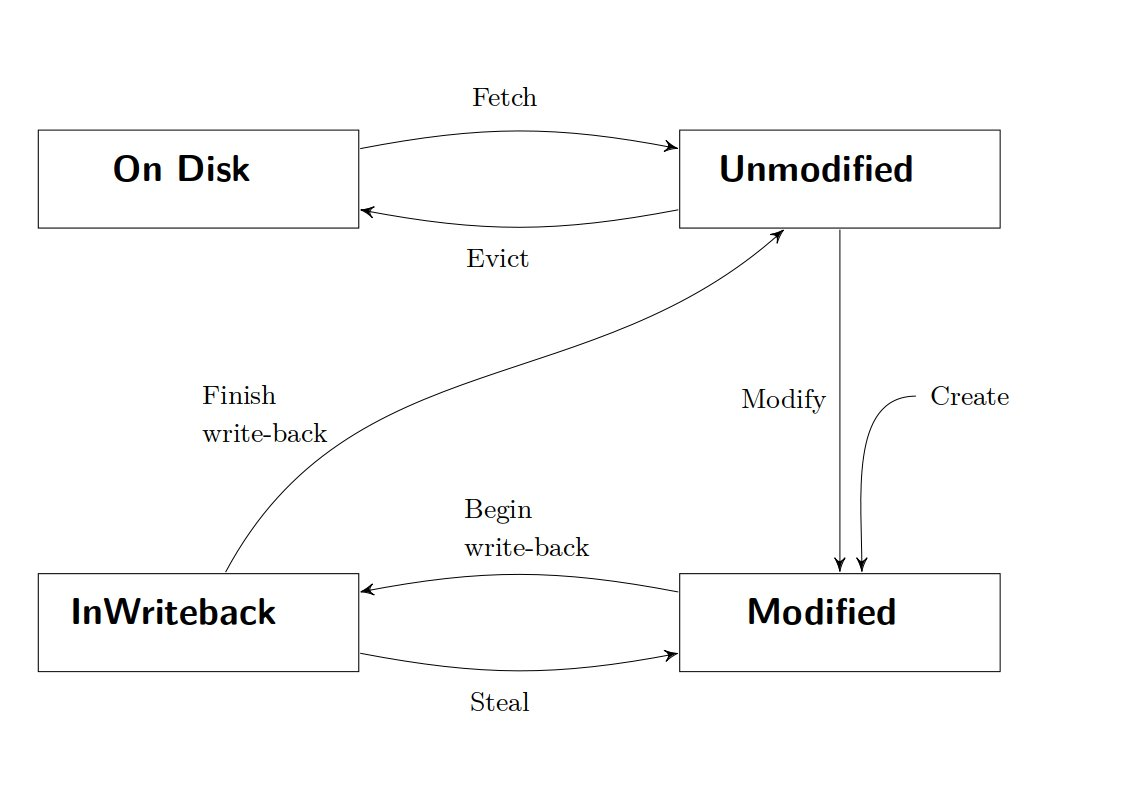
\includegraphics[scale=0.4]{DML_state_cycle.jpg}
	\caption{DML state cycle, \cite{wiedemann2018modern}}
		\label{fig:DML state cycle}
\end{figure}

The DMU manages the cache and the states of each \emph{ObjRef} as shown in \ref{fig:DML state cycle}.
The cycle starts with the creation of an object in modified state. When the DMU starts the write back of the object, the state
is changed to in write back state.
If the object is modified during write back through the steal function, it change the state back to modified.
When the write back is finished the object state change to unmodified.
An unmodified object can either change the state to modified if the object has been modified or evicted from cache to disk.
And lastly, any object on disk can be fetched in cache and will be in unmodified state.

For the cache, all objects are managed with an unique \emph{ObjectKey}, as shown in \ref{lst:ObjectKey enumeration}.
These \emph{ObjectKey} are  from the \emph{ObjRef} for each cache entry.
Objects in incomplete state are not stored in cache.

\bigskip

\begin{lstlisting}[language=Rust,mathescape=true,caption=ObjectKey enumeration,label=lst:ObjectKey enumeration]
pub enum ObjectKey<G> {
    Unmodified { offset: DiskOffset, generation: G },
    Modified(ModifiedObjectId),
    InWriteback(ModifiedObjectId),
}
\end{lstlisting}

\bigskip

\section{Cache Trait}

The DML state cycle and the fact that the cache is managed by the DMU place additional demands on the cache.
We see this in the cache trait, listing \ref{lst:simplified Cache trait}.

The first difference is that we have an explicit evict function. In most cache implementations, evict is a private function that the cache itself calls.
In our case, however, the DMU must call the evict function, not the cache itself.
Furthermore, the evict function must take into account that there are cache entries that 
are pinned i.e. in write back or modified state and therefore cannot be removed from the cache.
Also, the DMU can remove specific cache entries, listing  \ref{lst:simplified Cache trait} line 6 and line 7.
The \texttt{remove}()-function for unmodified entries and \texttt{force\_remove}() for pinned entries.

\bigskip

\begin{lstlisting}[language=Rust,mathescape=true,caption={simplified Cache trait without type aliases, generics, function parameters and function return types},label=lst:simplified Cache trait]
trait Cache {
    fn new();
    fn contains_key();
    fn get();
    fn get_mut();
    fn remove();
    fn force_remove();
    fn change_key();
    fn force_change_key();
    fn evict();
    fn insert();
    fn iter();
    fn $\textcolor{black}{\texttt{size}}$();
    fn capacity();
    fn stats();
    fn verify();
}
\end{lstlisting}

The second difference is that it must be possible to change the key for cache entries.
Because an object in cache can change his state 
Therefor we have two functions, listing \ref{lst:simplified Cache trait} line 8 and line 9. 
Again two functions for unmodified and pinned entries.

Another difference is that the cache must be able to handle cache entries of any size.
The handling of cache entries of arbitrary size is managed by the DMU.
Each fetched entry is always inserted into the cache, and then the eviction function is invoked until the cache capacity is again below the specified cache size.
So the cache size is a soft limit that can be temporarily exceeded, not a hard limit, which would mean that the eviction function is called
is called before inserting so that the cache size is never exceeded.

Furthermore, we have added the \texttt{get\_mut}()-function, \ref{lst:simplified Cache trait} line 5, 
since the \texttt{get}()-function does not allow that the state of the cache changes.
But this is needed for the implementation of ML-CLOCK, which we will discuss in more detail in section \ref{sub:ml-clock}.

\section{Implemented Cache Replacement Policies}
\label{sec:implemented cache replacement policies}
\subsection{CLOCK}

Clock cache was introduced by F.J.Corbató \cite{corbato1968paging} for the Multics operating system.
It is an approximation of the LRU (Least Recently Used) policy, but with a low runtime overhead, comparable to FIFO.

Unlike previous cache replacement algorithms, clock uses a circular list with a "hand" as a pointer to the current entry.
Each cache entry has a reference bit initialized to 0.
On a cache hit the reference bit for an entry is set to 1.
On a cache miss, we need an entry for eviction.
First, we look at the entry to which the hand is pointing. If the reference bit for this entry is 0, we have found the entry to be displaced.
If the reference bit is 1, we set the reference to 0 and move the pointer to the next entry.
These steps are repeated until we find an entry with an unset reference bit.

\newpage
% should try to get listing on one page, better to understand that way
\begin{lstlisting}[mathescape=true,caption=Clock replacement algorithm in pseudocode,label=lst:clock-algorithm]
$\textcolor{ovgu-blue}{Input}$
	Clk: Clock
	entry: entry on I/O request

if Clk.contains(entry) == true $\textcolor{ovgu-blue}{\texttt{then}}$
	// cache hit
	if entry.referenceBit == false $\textcolor{ovgu-blue}{\texttt{then}}$
		entry.referenceBit = true
	$\textcolor{ovgu-blue}{\texttt{end \ if}}$
else
	// cache miss
	if Clk.isFull() == true $\textcolor{ovgu-blue}{\texttt{then}}$
		// evict one entry
		while Clk.isFull() == true
			if Clk.hand.referenceBit == true $\textcolor{ovgu-blue}{\texttt{then}}$
				// second chance if reference bit was set
				Clk.hand.referenceBit = false
				Clk.hand = Clk.hand.next
			else
				// found entry for eviction 
				evict-candi = Clk.hand
				Clk.hand = Clk.hand.next
				Clk.evict(evict-candi)
			$\textcolor{ovgu-blue}{\texttt{end \ if}}$
		$\textcolor{ovgu-blue}{\texttt{end \ while}}$
	$\textcolor{ovgu-blue}{\texttt{end \ if}}$
	// insert entry to clock
	Clk.insert(entry)
$\textcolor{ovgu-blue}{\texttt{end \ if}}$	
return entry 
\end{lstlisting}

Clock also remove the lock contention problem of LRU.
For LRU each cache hit change the position of an entry in the LRU queue.
So cache hit have to be serialized behind a lock to be used in a parallel system.
Clock doesn't have this problem, because clock do not has to maintain an ordered queue.

Due to its simplicity and good performance in most cases, the clock algorithm is widely used for example in Linux, Windows and NetBSD.

 \todo[inline]{search for software which use clock as example with source}


\subsection{K-CLOCK}

Similar to normal clock algorithms but used a counter instead of just a bit for entry accesses.
The variable k can be chosen usually k=2 gives best performance.
Implemented in Haura with k=2.
Described in \cite{corbato1968paging} as a variation of the original clock algorithm.
K-Clock is similar to LRU-K as described in \cite{o1993lru} but clock-based not list-based.
It has the advantage that frequently accessed entries have a chance to stay longer in cache and new entries can leave the cache fast, leads to better performance in scan workloads.

\begin{lstlisting}[mathescape=true,caption=K-Clock replacement algorithm in pseudocode,label=lst:k-clock-algorithm]
$\textcolor{ovgu-blue}{Input}$
	Clk: Clock
	entry: entry on I/O request
	K: Number of max references stored per entry

if Clk.contains(entry) == true $\textcolor{ovgu-blue}{\texttt{then}}$
	// cache hit
	if entry.referenceCount < K $\textcolor{ovgu-blue}{\texttt{then}}$
		entry.referenceCount += 1
	$\textcolor{ovgu-blue}{\texttt{end \ if}}$
else
	// cache miss
	if Clk.isFull() == true $\textcolor{ovgu-blue}{\texttt{then}}$
		// evict one entry
		while Clk.isFull() == true
			if Clk.hand.referenceCount > 1 $\textcolor{ovgu-blue}{\texttt{then}}$
				// decrease reference count 
				Clk.hand.referenceCount -= 1
				Clk.hand = Clk.hand.next
			else
				// found entry for eviction 
				evict-candi = Clk.hand
				Clk.hand = Clk.hand.next
				Clk.evict(evict-candi}
			$\textcolor{ovgu-blue}{\texttt{end \ if}}$
		$\textcolor{ovgu-blue}{\texttt{end \ while}}$
	$\textcolor{ovgu-blue}{\texttt{end \ if}}$
	// insert entry to clock
	Clk.insert(entry)
$\textcolor{ovgu-blue}{\texttt{end \ if}}$
return entry 
\end{lstlisting}

\subsection{CLOCK-PRO}

Although the clock algorithm performs well in a variety of use cases, problems arise with weakly localized access patterns, as described in \cite{jiang2005making}.
Some problems include:
\begin{itemize}
	\item[1.] - access of many rarely used blocks can evict frequently used blocks for example in sequential scans
	\item[2.] - a loop pattern which is slightly larger then the cache 
	\item[3.] - in application with a B-tree index like databases, index blocks should be in cache but data blocks
				evict index blocks because of the shorter access time
\end{itemize}
% has been many alternative cache replacement algorithms LIRS is only one 
% could also mention more
% three categories of improvements
% 1. explicitly provide hints by user or programmer
% 2. detecting the access patterns failing LRU and switch to an other effective replacement strategie
% 3. using deeper history access information -> LIRS falls into this category

These problems are general problems for LRU base replacement algorithms.
An early attempt to overcome these problems was Low Inter-reference Recency Set (LIRS) \cite{10.1145/511399.511340} which uses the inter reference recency, the reuse distance, instead of last recency and divide the blocks in hot, with with low interreference recency and cold, with high inter-reference recency.
Unlike LRU, LIRS attempts to keep the hot blocks in the cache and remove only the cold blocks, to overcome the weaknesses of LRU in cases of weak locality.
To determine which blocks are hot or cold, LIRS also tracks metadata information for a set of cache blocks that are not resident in the cache.
LIRS uses a stack that includes hot, cold, and non-resident cold blocks, and an additional list for only resident cold entries.

Clock-Pro algorithm \cite{jiang2005clock} combines the efficiency from clock with the performance improvements from LIRS.
To achieve a better performance clock-pro combines LIRS stack and list in one circular list ordered by the last access.
Hot blocks, with small recencies are at the head of the list and cold blocks with large recencies are at the tail of the list.
After a cold block is insert into the clock, it is in a test period.
If an access during this test period occurs, the cold block become a hot block.
On the other hand if the cold block is not re-access during its test period, it will be removed.
It is possible that during the test period that the cold block will be removed from memory and became non-resident, then the meta data still remains in the clock until the cold block runs out of his test period.
So a non-resident cold block can when a re-access occurs, become a hot block.
To generate free space only resident cold blocks are evicted.

Clock-pro uses three handles instead of one like clock.
These three handles are used to determine the test-period and find an eviction candidate.
Since the test period, the threshold for an block to switch from cold to hot and also back from hot to cold is based on the distance between the handles the algorithm is adoptable and doesn't need a fixed threshold unlike other algorithms like CAR or 2Q.

\todo[inline]{insert image for clock-pro layout}

The hot-hand marks the tail of the list, which is the hot entry with the largest recency.
Any hot entry that would pass the hot hand is converted to a cold entry.
The cold-hand points to the last resident cold page and is used to find a replacement candidate for eviction.
The test-hand points to the last cold page in the test period. Any cold entry which passes this hand leaves the test period and any non-resident cold page in the test period that passes this pointer is removed from the clock.

\todo[inline]{make a diagram to show finding of eviction candidate}
\todo[inline]{decide if I want to use block, page or entry, shouldn't mix them up}
\newpage
\begin{lstlisting}[mathescape=true,caption=Clock-pro replacement algorithm in pseudocode,label=lst:clock-pro-algorithm]
$\textcolor{ovgu-blue}{Input}$
	Clk: Clock
	entry: entry on I/O request

if Clk.contains(entry) == true $\textcolor{ovgu-blue}{\texttt{then}}$
	// cache hit
	if entry.referenceBit == false $\textcolor{ovgu-blue}{\texttt{then}}$
		entry.referenceBit = true
	$\textcolor{ovgu-blue}{\texttt{end \ if}}$
else
	// cache miss
	if Clk.isFull() == true $\textcolor{ovgu-blue}{\texttt{then}}$
		while Clk.countHot + Clk.countCold >= Clk.capacity
			// run cold-hand to find evict candidate
			evict-candi = Clk.coldHand
			if evict-candi.coldBit == true $\textcolor{ovgu-blue}{\texttt{then}}$
				if evict-candi.referenceBit == true $\textcolor{ovgu-blue}{\texttt{then}}$
					// turn evict-candi to hot entry
					evict-candi.hotBit == true
					evict-candi.coldBit == false
					Clk.countHot += 1
					Clk.countCold -= 1
				else
					// turn resident Cold entry to non-resident Cold entry
					// only retain key and metadata
					Clk.turnNonResident(evict-candi)
					Clk.countCold -= 1
					Clk.countTest += 1	
				$\textcolor{ovgu-blue}{\texttt{end \ if}}$
			$\textcolor{ovgu-blue}{end \ if}$
			// move test hand if necessary
			while Clk.countTest > Clk.testCapacity
				// test hand turns resident cold entry to non-resident cold entry
				// if still in test-period
				entry = Clk.testHand
				if entry.testBit == true $\textcolor{ovgu-blue}{\texttt{then}}$
					Clk.testHand = Clk.testHand.next
					Clk.removeNonResidentEntry(entry)
					Clk.countTest -= 1
					if Clk.coldCapacity > 1
						Clk.coldCapacity -= 1
					$\textcolor{ovgu-blue}{\texttt{end \ if}}$
				$\textcolor{ovgu-blue}{\texttt{end \ if}}$
				Clk.testHand = Clk.testHand.next
			$\textcolor{ovgu-blue}{\texttt{end \ while}}$
			// move cold hand
			Clk.coldHand = Clk.coldHand.next
			// move hot hand if necessary
			while Clk.countHot > Clk.capacity - Clk.coldCapacity
				// hot hand removes reference bit on hot entry 
				// or turn not referenced hot entry to cold entry
				entry = Clk.hotHand
				if entry.hotBit == true $\textcolor{ovgu-blue}{\texttt{then}}$
					if entry.referenceBit == true $\textcolor{ovgu-blue}{\texttt{then}}$
						entry.referenceBit == false
					else
						entry.hotBit = false
						entry.coldBit = true
						Clk.countHot -= 1
						Clk.countCold += 1
					$\textcolor{ovgu-blue}{\texttt{end \ if}}$
				$\textcolor{ovgu-blue}{\texttt{end \ if}}$
				Clk.hotHand = Clk.hotHand.next
			$\textcolor{ovgu-blue}{\texttt{end \ while}}$
		$\textcolor{ovgu-blue}{\texttt{end \ while}}$
	Clk.insert(entry)
$\textcolor{ovgu-blue}{\texttt{end \ if}}$	
return entry 
\end{lstlisting}
\todo[inline]{maybe divide in two parts, eviction in own listing, it could be a bit long}

To make clock-pro adaptable the ratio for hot to cold entries is not fixed, unlike LIRS which has a fixed parameter for this.
It also influences if clock-pro behaves more like LRU and less like LIRS.
The cold-hand behaves like the hand in clock, unsetting reference bit and find eviction candidate.
If there are no hot entries clock-pro behaves like clock algorithm. 
However in case of where clock algorithm struggles, loop and scans, clock-pro can achieve better results.

If there are many entries with a small reuse distance (hot entries) and only a few cold entries. A new cold entry is evicted relatively quickly, but since it is still in the testing phase, it can be re-entered as a hot entry after an early re-access.
Hot entries also need more time before they are evicted because they must transform into cold entries before they are evicted.
For every cold page accessed during its test period we increment the capacity for cold pages by 1 and for every cold page which passes his test period without access we decrement the capacity by 1.
This will also adjust the speed  for cold- and hot-hand.

So clock-pro has the advantage of LRU in case of strong locality and better performance like LIRS in case of weak locality.


- problems with recursion
- show evict method 
- try to make evict method more understandable

\subsection{ML-CLOCK}
\label{sub:ml-clock}
%- newest algorithm of this three\\
%- based on single layer perceptron and online learning \\
%- also uses clock approach for efficient access compared to list based\\
%- also tries to minimize write back of entries\\
%- categorizes entries in clean (unchanged) and dirty (modified) entries\\
%- also tries to optimize write back by sort dirty entries by address in storage not by time \\
%- dirty entries can get second chance based on prediction by perceptron\\
%- perceptron lerns if LRU or LFU is more important \\

ML-clock \cite{cho2021ml} follows the recent trend to incorporate machine learning techniques.
what let ML-clock stand out is that it uses single-layer perceptron (SLP) which is a relatively simple ml technique.
But this allows the use of online learning instead of batch training which is used for neural networks and gives better adaptability.
It uses SLP to learn if it should behave more like LRU or LFU and incorporate learned I/O patterns.
Also ML-clock tries to minimize write operation and prioritize the eviction of clean entries instead of dirty entries.

ML-clock tries to reduce the number of access to the underlying storage media and incorporate machine learning techniques.
It starts with clock algorithm as basis. 
Unlike clock, ML-clock uses two hands.
Clean-hand to find eviction candidates which have not been modified and dirty-hand to find a modified eviction candidate.

To train the SLP we need to track the reference bit, reference count, and a timestamp for last access for every entry.
The reference bit is used just like in clock.
Reference count is to track the frequency of access and the timestamp for the recency.
SLP is used to decide which policies under the given circumstances is more suited.

To predict if an entry will be evicted the following equation is used.
The variables $w_d, w_c$ and $w_b$ represents the weight for reuse-distance, reference count and the bias.
The variables $x_d$ and $x_c$ represents the input values for reuse-distance and the reference count.

prediction: \\
\begin{align}
	f_{predict} (x_d, x_c) =
	\begin{cases}
		0, \quad x_d \cdot w_d + x_c \cdot w_c + 1 \cdot w_b < 0 \\
		1, \quad x_d \cdot w_d + x_c \cdot w_c + 1 \cdot w_b \geq 0
	\end{cases}
\end{align}

The variable $x_d$ must be reduced so that it has the same order of magnitude as $x_c$.
A prediction is triggered to find a victim page for eviction or to decide if a learning operation is triggered.

scaling of $x_d$:
\begin{align}
	x_d = \frac{current \  timestamp - timestamp \  of \  the \  last \  access}{size \  of \  circular \  list}
\end{align}
	
The variable $lr$ is the learning rate and controls how much the model change each epoch.
The equations below are used to train the new weights.
The learning operation is used to update the weights.

learning:
\begin{align}
\begin{split}
	w_d \leftarrow w_d + lr \cdot x_d \cdot (v_{expect} - v_{predict})\\
	w_c \leftarrow w_c + lr \cdot x_c \cdot (v_{expect} - v_{predict})\\
	w_b \leftarrow w_b + lr \cdot x_b \cdot (v_{expect} - v_{predict})
\end{split}
\end{align}

The variable $v_{predict}$ is the result of the prediction equations for a possible victim and 
$v_{expect}$ is the correct answer for this prediction.
The term $(v_{expect} - v_{predict})$ defines if the weights are updated or not.

In addition, ml-clock uses a ghost queue to store the metadata for eliminated entries in order to learn the weights.
The ghost queue can hold at most the same number of entries as the circular list.
Each time a new entry is added to the ghost queue and the ghost queue is full, a learning operation is triggered.
Useful because every evicted entries can be used to calibrate the SLP.

\newpage
\begin{lstlisting}[mathescape=true,caption=K-Clock replacement algorithm in pseudocode,label=lst:ml-clock-algorithm]
$\textcolor{ovgu-blue}{Input}$
	Clk: Clock
	hand: hand is the entry the clock hand is pointing to
	entry: entry on I/O request
	GhostQ: Ghost Queue

if Clk.contains(entry) == true $\textcolor{ovgu-blue}{then}$
	// trigger learning operation
	learning(entry, 1)
	return entry
else
	// cache miss
	if Clk.isFull() == true $\textcolor{ovgu-blue}{then}$
		// scan clean pages at the C-hand's location
		C-candi = Clk.findCleanCandidate()
		// scan dirty pages at the D-hand's location
		// in a sequential order (i.e, LBA)
		D-Candi = Clk.findDirtyCandidate()
		victim = prediction(C-candi, D-candi)
		// check if victim is in ghost queue
		if GhostQ.findPage(victim) == true $\textcolor{ovgu-blue}{then}$
			// ready to promote a entry to clock
			learning(entry, 1)
			GhostQ.deleteEntry(victim)
		else
			if GhostQ.isFull() == true $\textcolor{ovgu-blue}{then}$
				// evict a page on ghost queue with learning
				learning(GhostQ.tail, 0)
				GhostQ.deleteEntry(GhostQ.tail)
			$\textcolor{ovgu-blue}{end \ if}$
			GhostQ.insertEntry(victim)
		$\textcolor{ovgu-blue}{end \ if}$
		Clk.evict(victim)
	$\textcolor{ovgu-blue}{end \ if}$
	// insert entry to clock
	Clk.insert(entry)
$\textcolor{ovgu-blue}{end \ if}$
return entry 
\end{lstlisting}

\begin{table}[ht]
	\centering
	\begin{tabular}{|c|c|c|}
		\hline
		\textbf{Predicted Value} & \textbf{Predicted Value} & \textbf{Victim Entry} \\
		\textbf{(C-Candidate)} & \textbf{(D-Candidate)} & \\
		\hline
		0 & 0 & C-Candidate \\
		\hline
		0 & 1 & C-Candidate \\
		\hline
		1 & 0 & D-Candidate \\
		\hline
		1 & 1 & C-Candidate \\
		\hline
	\end{tabular}
	\caption{Preference rules for victim entry}
	\label{tab:ml-clock preference rules}
\end{table}


- two separated clocks one for clean entries one for dirty and also order by block address \\
- lock needed for get function because entry can change clock

\section{Usage}
- code changes for compilation of haura with different cache\\
- how to compile haura with different cache implementation \\
%To implement different cache policies we need to modify src/database/mod.rs.
%Because there the DMU will be created.
%Used conditional compilation see Cargo.toml to build with different cache default is CLOCK.

\section{Summary}

\chapter{Evaluation}
\label{cha:evaluation}

% detalierte Beschreibung des Testsystems und der Testumgebung, Software Hardware etc.
% soll reproduzierbar sein
% Wie soll man die Daten angeben reicht Diagramme?
% was sind die Kriterien für die Evaluation, Latenz, Cache-misses, Ausführungszeit, ...
% Interpretation der Resultate
% Vorteile und Nachteile darstellen

% 25-35%, ca. 10-14 Seiten

-> start after benchmarks are done

% possible structure
\section{Setup}

- used ovgu cluster
- software version 
- haura config json


\section{Methodology}
- synthetic benchmarks with fio zipf and random, if I get random to work\\
- zip benchmark with linux kernel source files\\
% \cite{karakostas2000practical} -> contains zipfian distribution as use case for webcaches
- only synthetic benchmarks 
- zipf, normal, zoned, uniform 

\section{Results}

- problems with results, capacity management doesn't work in all cases

\section{Summary}

\chapter{Conclusion}
\label{cha:conclusion}
% could be conclusions and future work

\section{Future Work}

-> after evaluation

% 5-10%, 2-5 Seiten


\bibliographystyle{apalike}
\bibliography{thesis}

% \backmatter
% should be around 20 references for bachelor thesis
% avoid to cite web sites


\appendix

%\chapter{Appendix}
%\label{cha:appendix}

% could also be ad the beginning
% implement acronyms or list of Abbreviations

%\setcounter{tocdepth}{1}
%\listoffigures
%\setcounter{tocdepth}{1}
%\listoftables
%\lstlistoflistings

\chapter*{}

\section*{Statement of Authorship}

I herewith assure that I wrote the present thesis independently, that the thesis has not been partially or fully submitted as graded academic work and that I have used no other means than the ones indicated.
I have indicated all parts of the work in which sources are used according to their wording or to their meaning.

I am aware of the fact that violations of copyright can lead to injunctive relief and claims for damages of the author as well as a penalty by the law enforcement agency.

\bigskip

Magdeburg, \today

\bigskip
\bigskip

\rule{0.5\textwidth}{0.5pt}\\
\hspace*{0.25em}Signature

\end{document}

%-> can start with this chapter when I decide which benchmark and metrics I want to use\\
%- fio for synthetic benchmarks -> zipf dis. and sequential should be covered\\
%- try to find traces which I can use easily \\
%- some articles uses SPEC-Benchmark traces\\
%
%- general problem that we are dealing with variable sized cache entries and also \\
%  pinning an entry is possible which increases the difficulty of implementation of most suggested algorithms\\
%- most algorithms based an equally sized pages/entries without pinning\\
%- ml-clock with extra locking which could lead to problems, clock and clock-pro uses atomics to prevent this

